%%%%%%%%%%%%%%%%%%% - ANEXOS - %%%%%%%%%%%%%%%%%%%

\newpage
\section*{ANEXOS} \label{sec:anexos} % Se añade un asterisco a \section para que el título no esté numerado.
\phantomsection
\addcontentsline{toc}{section}{ANEXOS} % Al utilizar \section* se ha de añadir manualmente el apartado al índice (Table Of Contents, TOC).
\markright{ANEXOS} % Al utilizar \section* se ha de añadir manualmente el título del apartado al encabezado.

\renewcommand{\thesubsection}{\Alph{subsection}} % Se numeran los anexos con letras del alfabeto en lugar de números.
% Se indica que las tablas, figuras y códigos se numeran con el código del anexo (A, B, C, ...) seguido del número de tabla, figura o código dentro del anexo (tabla A.2, figura C.1, etc.)
\renewcommand{\thetable}{\Alph{subsection}.\arabic{table}}
\renewcommand{\thefigure}{\Alph{subsection}.\arabic{figure}}
\renewcommand{\thecode}{\Alph{subsection}.\arabic{code}}

% ---------------- Primer anexo ---------------- %
\setcounter{subsection}{0}
\setcounter{table}{0}
\setcounter{figure}{0}

\subsection{Gráficas obtenidas en la segunda simulación larga fallida} \label{graficas_erroneas}

\textit{Simulación de 6 horas y 40 minutos realizada en el \acrshort{sgiz} el 30 de abril de 2024.}

A continuación, se muestran algunas de las gráficas obtenidas en la simulación fallida explicada en el apartado \ref{sim_larga_fallida}, con una estabilización incorrecta a partir de las 4 horas:

\begin{figure}[!h]
    \centering
    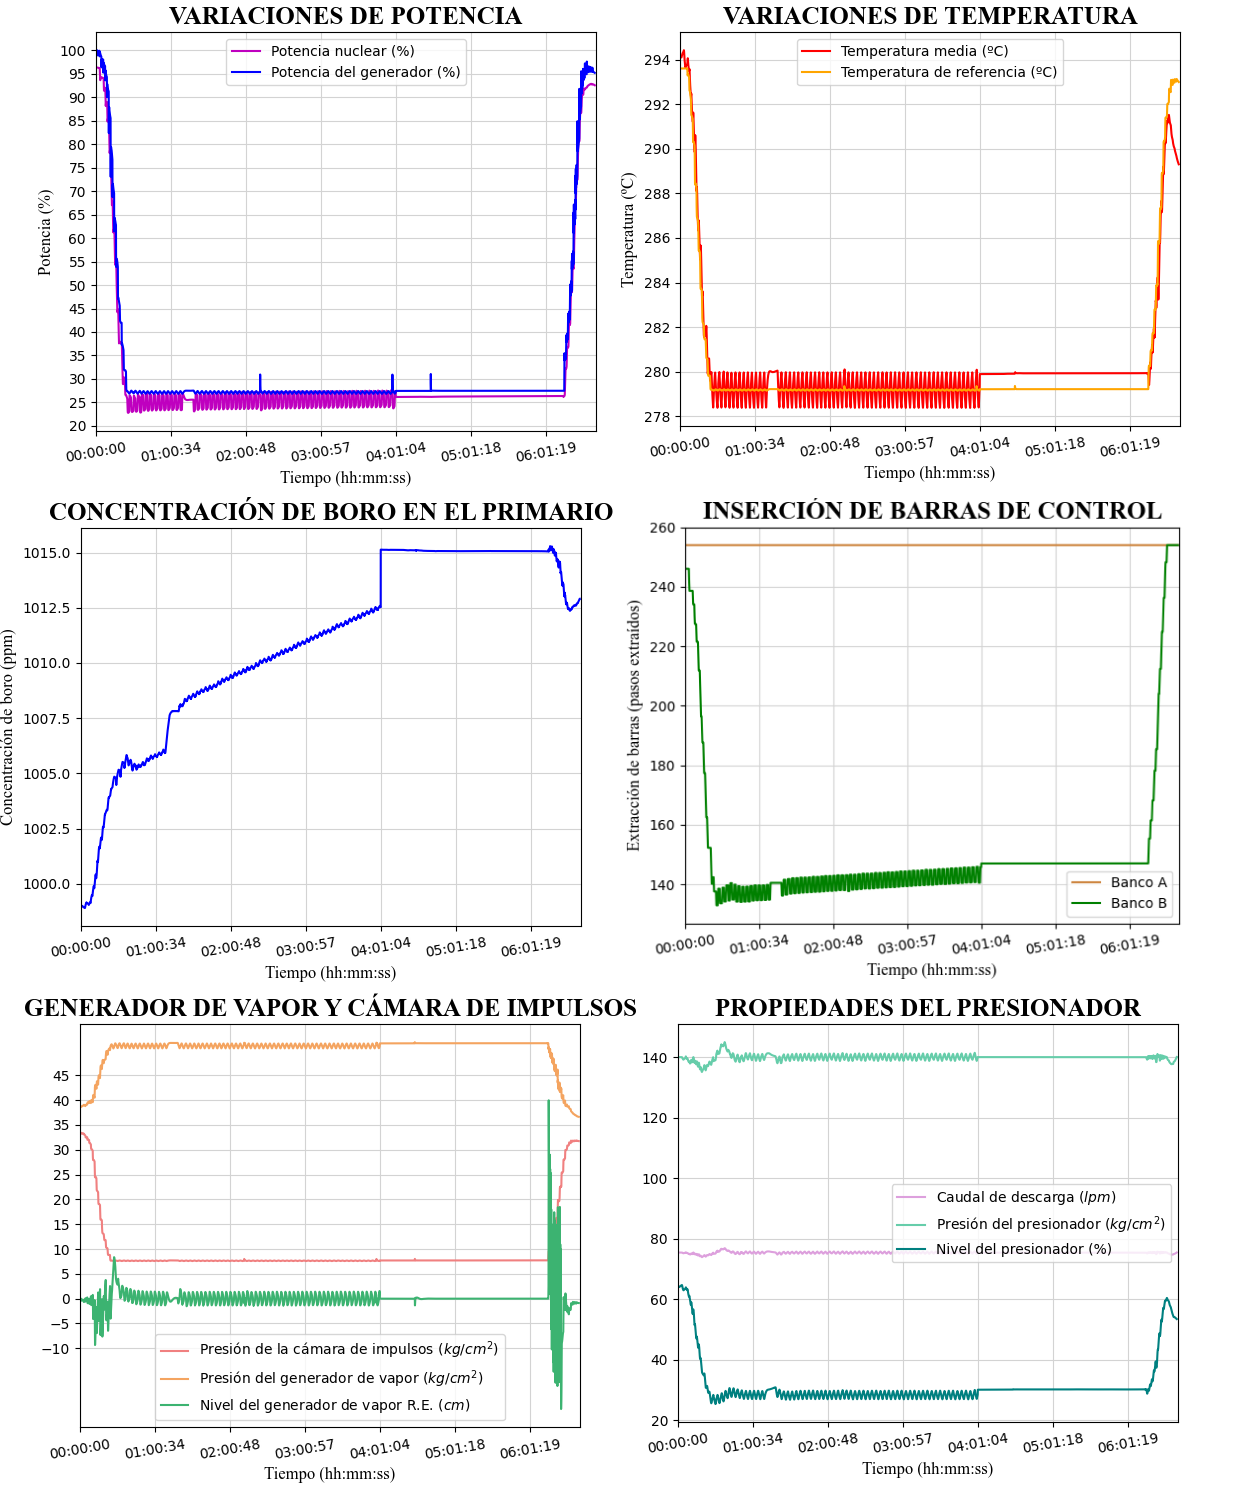
\includegraphics[width=\textwidth]{content/figures/sim2_peque.png}
    \caption{Gráficas imperfectas de la segunda simulación larga fallida.}
    \label{fig:sim2_peque}
\end{figure}

\newpage
\subsection{Resultados de la encuesta de la práctica} \label{resultados_encuesta_practica}

Tal y como se comenta en el apartado \ref{feedback_practica}, tras la realización de la práctica de seguimiento de carga en el \acrshort{sgiz} por parte de 28 alumnos de la asignatura de \textit{Tecnologías Avanzadas en Reactores Nucleares} del máster, se envió una encuesta para obtener retroalimentación sobre la sesión. A continuación, se muestran los resultados detallados de las 12 respuestas obtenidas:

\begin{enumerate}
    \item \textbf{¿Habías hecho alguna práctica similar en el \acrshort{sgiz} anteriormente?}
    
    \begin{figure}[!h]
        \centering
        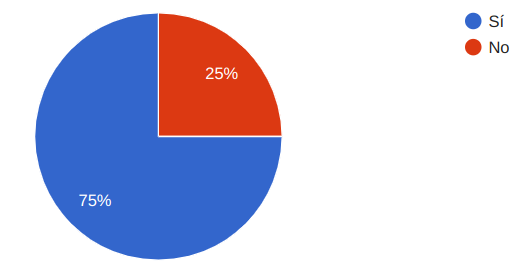
\includegraphics[width=0.47\textwidth]{content/figures/encuesta_1.png}
        \caption{Resultados pregunta 1.}
        \label{fig:encuesta_1}
    \end{figure}

    \item \textbf{¿Crees que la práctica se enmarca adecuadamente en la asignatura de Tecnologías Avanzadas en Reactores Nucleares?}
    
    \begin{figure}[!h]
        \centering
        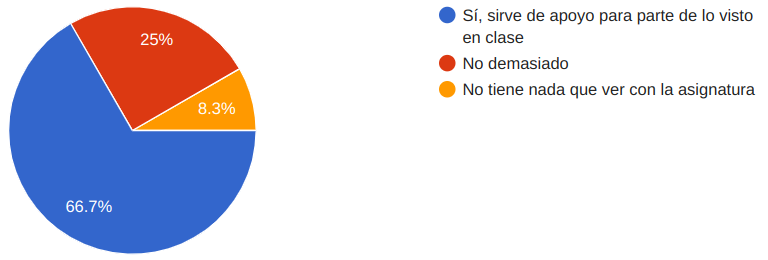
\includegraphics[width=0.72\textwidth]{content/figures/encuesta_2.png}
        \caption{Resultados pregunta 2.}
        \label{fig:encuesta_2}
    \end{figure}
    
    \item \textbf{¿Habías oído hablar antes de las capacidades avanzadas de seguimiento de carga para las que se diseñan los \acrlongpl{smr}?}
    
    \begin{figure}[!h]
        \centering
        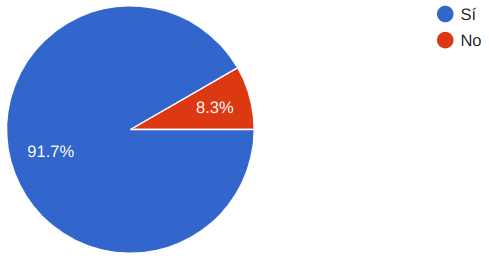
\includegraphics[width=0.47\textwidth]{content/figures/encuesta_3.png}
        \caption{Resultados pregunta 3.}
        \label{fig:encuesta_3}
    \end{figure}
    
    \newpage
    \item \textbf{¿Has aprendido cosas nuevas con la práctica?}
    \newline
    \begin{figure}[h]
        \centering
        \vspace{-0.5cm}
        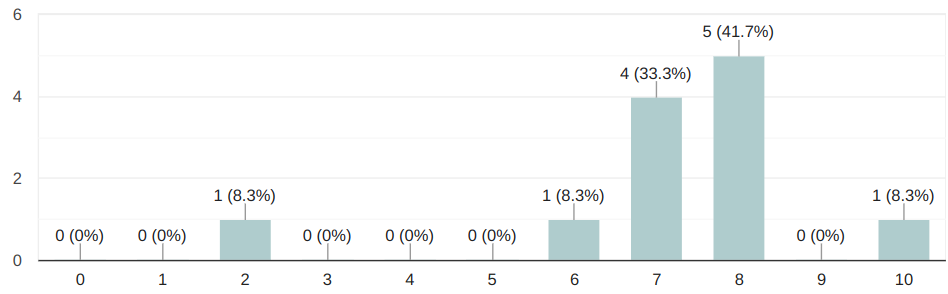
\includegraphics[width=\textwidth]{content/figures/encuesta_4.png}
        \caption{Resultados pregunta 4.}
        \label{fig:encuesta_4}
    \end{figure}
    
    \item \textbf{¿Te ha ayudado a comprender mejor las características y el funcionamiento general de los principales componentes y sistemas del reactor durante la operación del mismo?}
    
    \begin{figure}[h]
        \centering
        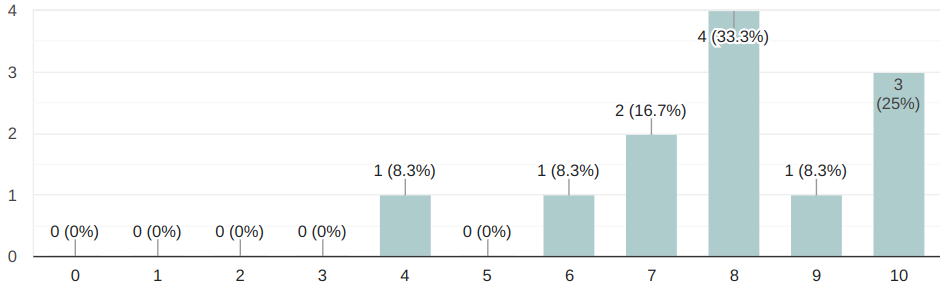
\includegraphics[width=\textwidth]{content/figures/encuesta_5.png}
        \caption{Resultados pregunta 5.}
        \label{fig:encuesta_5}
    \end{figure}
    
    \item \textbf{¿Se han entendido bien el objetivo, el procedimiento y las conclusiones de la simulación realizada? ¿Las explicaciones han sido suficientemente claras?}
    
    \begin{figure}[!h]
        \centering
        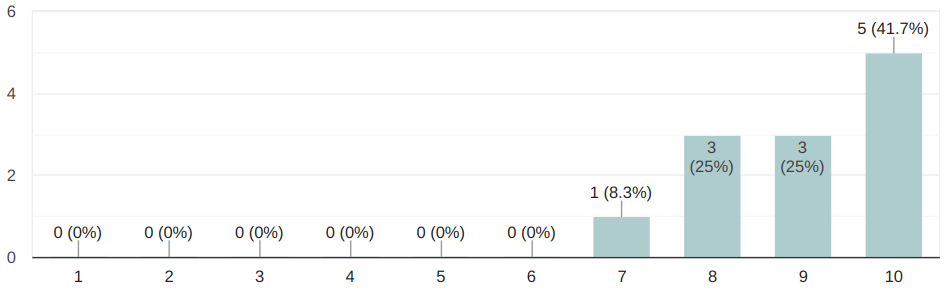
\includegraphics[width=\textwidth]{content/figures/encuesta_6.png}
        \caption{Resultados pregunta 6.}
        \label{fig:encuesta_6}
    \end{figure}
    
    \newpage
    \item \textbf{En general, ¿crees que realizar prácticas en el simulador ayuda a entender mejor lo visto en algunas asignaturas del grado y del máster?}
    
    \begin{figure}[!h]
        \centering
        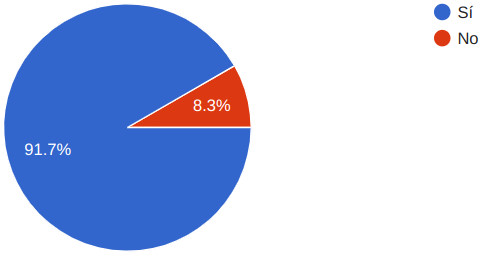
\includegraphics[width=0.47\textwidth]{content/figures/encuesta_7.png}
        \caption{Resultados pregunta 7.}
        \label{fig:encuesta_7}
    \end{figure}

    \item \textbf{Finalmente, valora del 0 al 10 tu grado de satisfacción general con la práctica realizada:}
    
    \begin{figure}[!h]
        \centering
        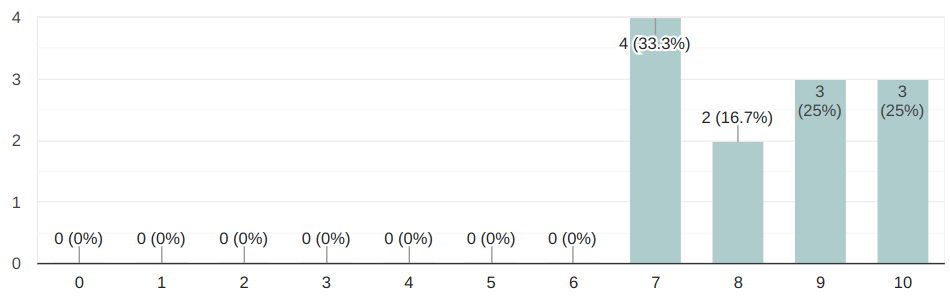
\includegraphics[width=\textwidth]{content/figures/encuesta_8.png}
        \caption{Resultados pregunta 8.}
        \label{fig:encuesta_8}
    \end{figure}
\end{enumerate}

Además de las 8 preguntas mostradas, se añadió una sección en el formulario para que los alumnos hicieran comentarios adicionales. La información aportada en esa sección es de gran utilidad y se encuentra resumida en el apartado \ref{feedback_practica}.

\newpage
\subsection{Código} \label{sec:codigo}

Todas las gráficas de las simulaciones realizadas en el \acrshort{sgiz} han sido elaboradas con \textit{Python} a partir de los datos generados en \textit{Excel} por el propio simulador. A continuación, se muestra, a modo de ejemplo, el código para la obtención de una de las gráficas:

\vspace{-5pt}

\begin{code}[H]
\begin{lstlisting}[firstnumber=1, breakindent=55pt]
  # Importación de las librerías necesarias
  import matplotlib.pyplot as plt
  import numpy as np
  import pandas as pd

  # Obtención de datos:
  gen_vapor_camara_imp=pd.read_excel("simulacion3.xlsx","gen_vapor_camara_imp")
  df_gen_vapor_camara_imp=pd.DataFrame=gen_vapor_camara_imp

  tiempo=[]
  for i in range(0,len(df_gen_vapor_camara_imp.tiempo)):
      tiempo.append(df_gen_vapor_camara_imp.tiempo[i].strftime('%H:%M:%S'))
    
  pres_cam_imp=[]
  for i in range(0,len(df_gen_vapor_camara_imp.pres_cam_imp)):
      pres_cam_imp.append(df_gen_vapor_camara_imp.pres_cam_imp[i])

  presion_gen_vapor=[]
  for i in range(0,len(df_gen_vapor_camara_imp.               presion_gen_vapor)):
      presion_gen_vapor.append(df_gen_vapor_camara_imp.presion_gen_vapor[i])

  nivel_gen_vapor=[]
  for i in range(0,len(df_gen_vapor_camara_imp.nivel_gen_vapor)):
      nivel_gen_vapor.append(df_gen_vapor_camara_imp.nivel_gen_vapor[i])

  # Creación del gráfico
  plt.plot(tiempo, presion_camara_impulsos, label='Presión de la cámara de impulsos $(kg/cm^2)$', color='lightcoral')
  plt.plot(tiempo, presion_gen_vapor, label='Presión del generador de vapor $(kg/cm^2)$', color='sandybrown')
  plt.plot(tiempo, nivel_gen_vapor, label='Nivel del generador de vapor R.E. $(cm)$', color='mediumseagreen')

  # Creación de la leyenda y el título
  plt.legend(loc='best')
  plt.xlabel('Tiempo (hh:mm:ss)', family='Times New Roman', size=12)
  plt.title('COMPORTAMIENTO GENERADOR DE VAPOR Y CÁMARA DE IMPULSOS', fontname='Times New Roman', size=18, weight='bold')
  plt.grid(True, color='lightgrey')
  plt.yticks(np.arange(-10,50,5))
  plt.xlim([0, len(tiempo)])
  plt.xticks(np.arange(0,len(tiempo),360))
  plt.xticks(rotation = 10)

  # Mostrar el gráfico
  plt.show()
\end{lstlisting}
\vspace{-5pt}
\caption{Ejemplo del código utilizado para generar las gráficas de las simulaciones. Este en concreto corresponde al código de la figura \ref{fig:sim3_gen_vapor_camara_imp}.}
\label{cod:codigo_graficas}
\end{code}